\chapter{Computation Time for Kociamba's Optimal Solver}
\label{app:kociembaTime}
\myTop{In order to determine the time efficiency of  Kociemba's optimal solver, we have computed a test.}
In order to calculate the time used to solve a \rubik{} using Kociemba's optimal solver, we have gathered data from our application in form of time stamps when ever the solver has finished a search depth.

The data was gathered on a 2.5 GHz Intel Duo Core processor (P9500) with 4 GB RAM running on Linux-Ubuntu v. 10.04.
The data gathered with these specifications are shown in table \ref{tab:timeData}.

\begin{table}[hb]
\centering
	\begin{tabular}{|l|l|}
	\hline
	Search depth&Time to finish[ms]\\
	\hline
	0&2\\
	\hline
	1&4\\
	\hline
	2&14\\
	\hline
	3&74\\
	\hline
	4&432\\
	\hline
	5&1775\\
	\hline
	6&19921\\
	\hline
	7&289744\\
	\hline
	8&4339435\\
	\hline
	\end{tabular}
\caption{\myCaption{Data for computation time of Kociemba's optimal solver}}
	\label{tab:timeData}
\end{table}

To make the approximation we assume that the time will evolve exponentially based on figure \ref{fig:timeFunction}.

\begin{figure}[tbh]
	\centering
		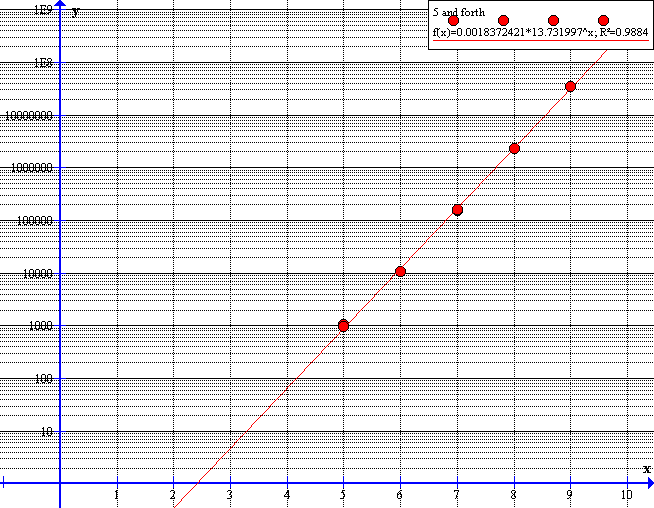
\includegraphics[scale=0.5]{input/pics/timeFunction}
	\caption{\myCaption{The approximation of the time needed to finish the search depth. It is displayed on a logarithmic y-axis to show that an exponential function seem to fit.}}
	\label{fig:timeFunction}
\end{figure}

The figure shows the last four data points since the first five are inaccurate due to small amount time which means that other processes might have interferred with the computation time.

As figure \ref{fig:timeFunction} shows the function for calculating the time needed to finish the search depth $x$ is:
\[
f(x)=0.0035413937 \cdot 13.575029^{x} ms
\]
The $R^2$ is close to 1 and this tell us that the approximation is relativly good. Especialy for calculating this; where the precision is not essential.

We are interrested in approximating the time that it would take to solve a \rubik{}. Since the average \rubik{} needs 18 moves to solve \cite{kociemba09} we will estimate the time to compute this:
\[
f(18) = 0.0035413937 \cdot 13.575029^{18} \approx 8.6798 \cdot 10^{17} ms \approx 27523465 years
\]

\myTail{TAIL}